% !TEX program = XeLaTeX
%----------------------------------------------------------------------------------------
%	PACKAGES
%----------------------------------------------------------------------------------------
\documentclass[hyperref={pdfpagelabels=false}]{beamer}
\usepackage[orientation=portrait,size=a0,scale=1.4]{beamerposter}
\usepackage[font={small}]{caption}
\usepackage[english]{babel}
\usepackage{fontspec, xcolor, tikz, algorithm, algpseudocode, csvsimple, tabularx, rotating, wrapfig}

%----------------------------------------------------------------------------------------
%	DOCUMENT CONFIGURATIONS
%----------------------------------------------------------------------------------------
\usetheme{NTNU}

\setlength{\paperwidth}{33.1in}
\setlength{\paperheight}{46.8in}

\captionsetup{skip=0pt, belowskip=0pt, aboveskip=0pt, font=small}
\setbeamertemplate{caption}[numbered]

\setmainfont[
  Path=resources/fonts/,
  Extension=.ttf,
  BoldFont=*bd,
  ItalicFont=*i,
  BoldItalicFont=*bi
]{arial}
\setsansfont[
  Path=resources/fonts/,
  Extension=.ttf,
  BoldFont=*bd,
  ItalicFont=*i,
  BoldItalicFont=*bi
]{arial}

\newlength\origleftmargini
\setlength\origleftmargini\leftmargini
\setbeamertemplate{itemize/enumerate body begin}{\setlength{\leftmargini}{1.2em}}

\definecolor{mydark}{HTML}{232834}

%----------------------------------------------------------------------------------------
%	TITLE SECTION
%----------------------------------------------------------------------------------------
\listfiles

\title{\Huge{Feasibility Study of Social Network Analysis on Loosely Structured Communication Networks}}

\author{Jan William Johnsen and Katrin Franke}

\institute{jan.w.johnsen@ieee.org and kyfranke@ieee.org}

%----------------------------------------------------------------------------------------

\begin{document}

\addtobeamertemplate{block end}{}{\vspace*{1ex}} % White space under blocks

\begin{frame}[fragile] % The whole poster is enclosed in one beamer frame

%\vspace{0em}

\begin{columns}[t]

%----------------------------------------------------------------------------------------
%	FIRST COLUMN
%----------------------------------------------------------------------------------------
\begin{column}{.052\textwidth}\end{column} % Empty spacer column

\begin{column}{.45\textwidth} % The first column

%	HIGHLIGHTS
%----------------------------------------------------------------------------------------
\begin{block}{Highlights}
  \begin{itemize}
    \item Organised criminal groups become more active in the cyber domain, where they form online communities used as marketplaces for illegal material, products and services purchased by other criminals.
    \item Trading of illegal goods drives an underground economy that facilitates almost any type of cyber crime. The challenge for law enforcement agencies is to know which individuals to focus their efforts on, in order to effectively disrupt the marketplaces.
    \item Our article study the feasiability of using \textbf{social network analysis} on loosely structured communication networks with the goal of identifing central individuals who provide services to cyber criminals.
  \end{itemize}
\end{block}


%	METHODOLOGY
%----------------------------------------------------------------------------------------
\begin{block}{Case study methodology}
  \begin{itemize}
    \item Social network analysis studies social relationships through the use of network graphs. In these graphs, \textbf{vertices} are individual actors and \textbf{edges} are the relationships between them.
    \item \textbf{Centrality measures} identify important and influential individuals in a network. These measures often differ in their evaluation of vertex importance.
  \end{itemize}

  \begin{figure}[H]
  	\begin{minipage}{0.48\columnwidth}
  		\centering
  		\includegraphics[width=0.99\columnwidth]{../pdf/degree_centrality}
  		\caption{Highlighting largest degree centrality}
  		\label{fig:degree_centrality}
  	\end{minipage}
  	~
  	\begin{minipage}{0.48\columnwidth}
  		\centering
  		\includegraphics[width=0.99\columnwidth]{../pdf/betweenness_centrality}
  		\caption{Highlighting largest betweenness centrality}
  		\label{fig:betweenness_centrality}
  	\end{minipage}
  \end{figure}

  \begin{figure}[H]
  	\begin{minipage}{0.48\columnwidth}
  		\centering
  		\includegraphics[width=0.99\columnwidth]{../pdf/closeness_centrality}
  		\caption{Highlighting largest closeness centrality}
  		\label{fig:closeness_centrality}
  	\end{minipage}
  	~
  	\begin{minipage}{0.48\columnwidth}
  		\centering
  		\includegraphics[width=0.99\columnwidth]{../pdf/eigenvector_centrality}
  		\caption{Highlighting largest eigenvector centrality}
  		\label{fig:eigenvector_centrality}
  	\end{minipage}
  \end{figure}
\end{block}

%	CASE STUDY DESIGN
%----------------------------------------------------------------------------------------
\begin{block}{Case study and novel hacker forum dataset}
  \begin{itemize}
    \item A novel dataset from \textbf{Nulled.IO} was leaked on 12/05/2017. It is from an online forum for distributing cracked software and leaked credentials.
    \item The database dump contains details for about 600 000 users, including around 800 000 private and 3.5 million public messages.
    \item Two networks – modelled by \textbf{undirected graphs} – were created to model both private and public communciations.
  \end{itemize}
  \begin{figure}
    \colorbox{mydark}{
\includegraphics[scale=1.2]{figures/nulled.png}}
    %\caption{Nulled.IO logo}
    %\label{fig:Nulled.IO logo}
  \end{figure}
\end{block}

\begin{block}{Centrality measures results}
  \begin{table}[!ht]
    \footnotesize
    \caption{Top ten public centrality results}
  	\label{tab:app_undirected_sna_results_top_10_public}
    \begin{tabular}{| l | l || l | l || l | l || l | l |}
  		\hline
  		\textbf{ID} & \textbf{Degree} & \textbf{ID} & \textbf{Closeness} & \textbf{ID} & \textbf{Betweenness} & \textbf{ID} & \textbf{Eigenvector} \\ \hline
  		\csvreader[head to column names,late after line=\\]{../data/sna_results_threads_10_threshold_1.csv}{}
  		{\eidone & \degree & \eidtwo & \closeness & \eidthree & \betweenness & \eidfour & \eigenvector}
  		\hline
  	\end{tabular}
  \end{table}
\end{block}

\end{column}

%----------------------------------------------------------------------------------------
%	SECOND COLUMN
%----------------------------------------------------------------------------------------
\begin{column}{.01\textwidth}\end{column} % Empty spacer column

\begin{column}{.45\textwidth} % The second column

%	RESULTS
%----------------------------------------------------------------------------------------
\begin{exampleblock}{}
  \begin{table}[!ht]
  \footnotesize
  	\caption{Top ten private centrality results}
  	\label{tab:app_undirected_sna_results_top_10_private}
  	\begin{tabular}{| l | l || l | l || l | l || l | l |}
  	  \hline
  	  \textbf{ID} & \textbf{Degree} & \textbf{ID} & \textbf{Closeness} & \textbf{ID} & \textbf{Betweenness} & \textbf{ID} & \textbf{Eigenvector} \\ \hline
  	  \csvreader[head to column names,late after line=\\]{../data/sna_results_pm_10_threshold_1.csv}{}
  	  {\eidone & \degree & \eidtwo & \closeness & \eidthree & \betweenness & \eidfour & \eigenvector}
  	  \hline
  	\end{tabular}
  \end{table}
\end{exampleblock}

%	RESULTS
%----------------------------------------------------------------------------------------
\begin{block}{Network visualisation}
  \begin{figure}[!ht]
  	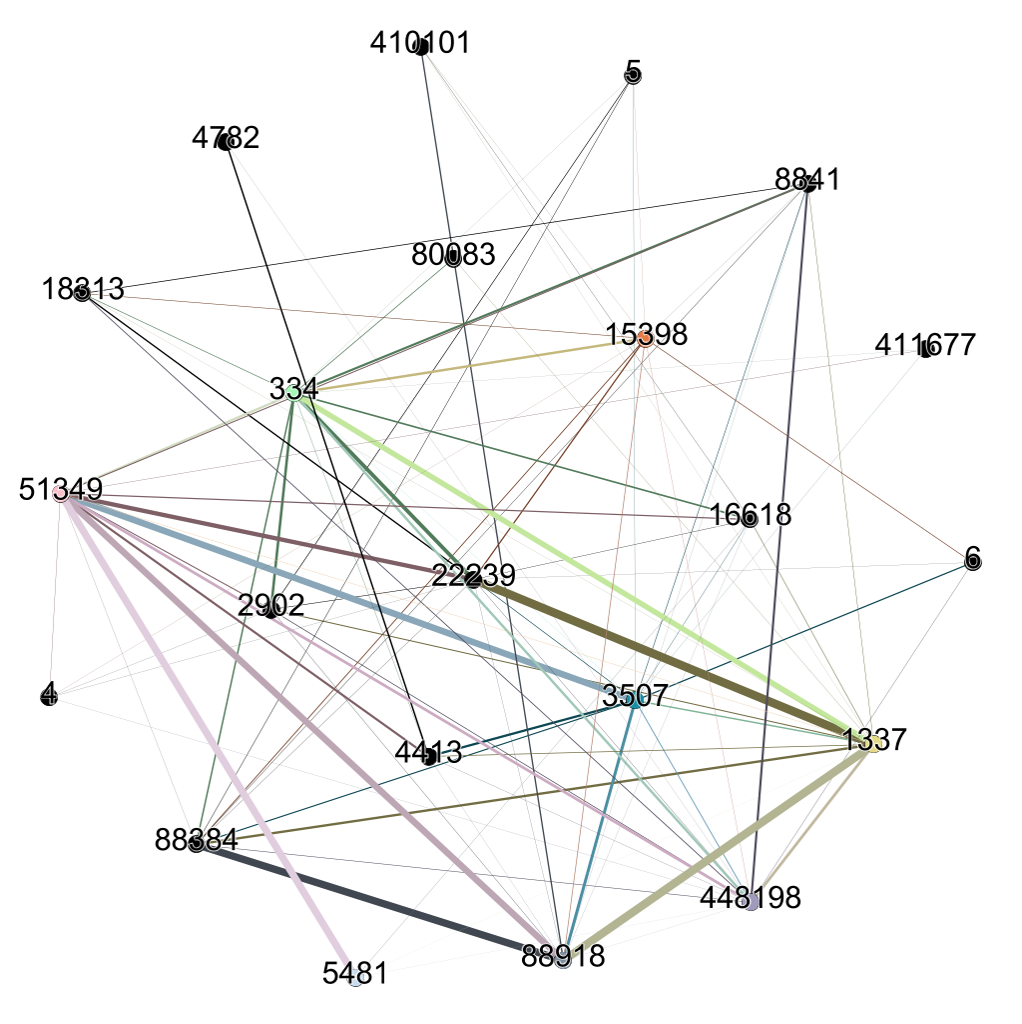
\includegraphics[width=0.65\textwidth]{figures/public_threads_network.png}
  	\caption{Public threads}
  	\label{fig:public_threads_visualisation}
  \end{figure}

  \begin{figure}[!ht]
  	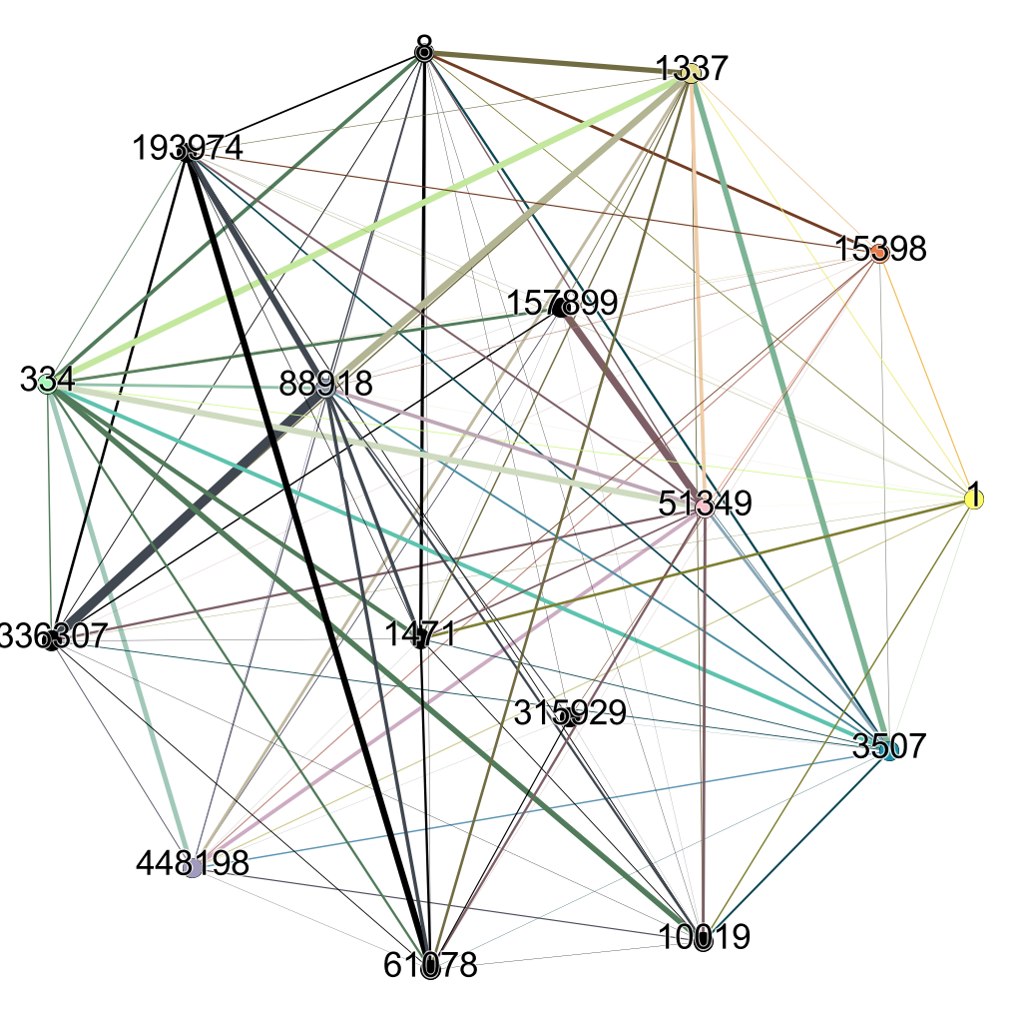
\includegraphics[width=0.65\textwidth]{figures/private_messages_network.png}
  	\caption{Private messages}
  	\label{fig:private_messages_visualisation}
  \end{figure}
\end{block}

%	SUMMARY
%----------------------------------------------------------------------------------------
\begin{block}{Summary}
  \begin{itemize}
    \item Centrality measures ranked administrators as more important than cyber criminals who provide illegal services to others. Focusing on disrupting server administrators is an inefficient approach addressing this problem, as their removal represents only a temporarily setback for prolific cyber criminal networks.
  \end{itemize}
  \begin{figure}
    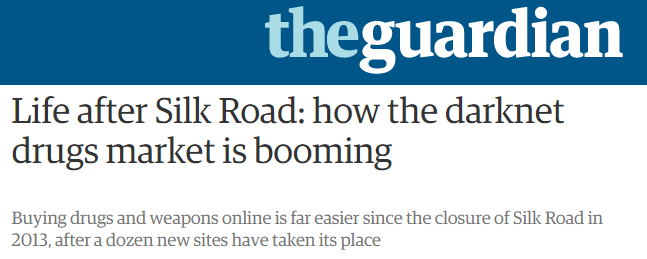
\includegraphics[scale=1.4]{figures/theguardian.png}
    %\caption{Screen capture of Guardian article}
    %\label{fig:Guardian article}
  \end{figure}
\end{block}

%	REFERENCES
%----------------------------------------------------------------------------------------
%\begin{block}{References}
%\bibliographystyle{alpha}
%\scriptsize{
%  \bibliography{references}
%}
%\end{block}

\end{column} % End of the second column

\begin{column}{.039\textwidth}\end{column} % Empty spacer column

\end{columns} % End of all the columns in the poster

\end{frame}

\end{document}
